% WIP
% 
% This document was inspired by a Template by Akash Benerjee: https://www.overleaf.com/articles/akash-banerjees-cv/qcxhvqqybqrq
% Feel free to distribute this template, but please keep the
% referal to HowToTeX.com.
% Date: May 2019
%%%%%%%%%%%%%%%%%%%%%%%%%%%%%%%%%%%%%%%%%%%%%%%%%%%%%%%%%%%%%%%%%%%%%%
\documentclass[paper=a4,fontsize=11pt]{scrartcl} % KOMA-article class
							
\usepackage[english]{babel}
\usepackage[utf8x]{inputenc}
\usepackage[protrusion=true,expansion=true]{microtype}
\usepackage{amsmath,amsfonts,amsthm}     % Math packages
\usepackage{graphicx}                    % Enable pdflatex
\usepackage[svgnames]{xcolor}            % Colors by their 'svgnames'
\usepackage{geometry}
	\textheight=700px                    % Saving trees ;-)
\usepackage{url}
\usepackage{sectsty}

\frenchspacing              % Better looking spacings after periods
\pagestyle{empty}           % No pagenumbers/headers/footers

%%% Macros
%%% ------------------------------------------------------------
\newlength{\spacebox}
\settowidth{\spacebox}{8888888888}			% Box to align text
\newcommand{\sepspace}{\vspace*{1em}}		% Vertical space macro

\newcommand{\MyName}[1]{ % Name
  \Huge \usefont{OT1}{phv}{b}{n} \hfill #1
  \par \normalsize \normalfont}

\newcommand{\MySlogan}[4]{ % Slogan (optional)
  \large \usefont{OT1}{phv}{m}{n}\hfill \textit{#1} 
  \sepspace
  \par \normalsize \usefont{OT1}{phv}{m}{n}\hfill \textit{#2}
  \par \normalsize \usefont{OT1}{phv}{m}{n}\hfill \textit{#3}
  \par \normalsize \usefont{OT1}{phv}{m}{n}\hfill \textit{#4}
  \par \normalsize \normalfont}

%%% Document
%%% ------------------------------------------------------------
\begin{document}
  
  \MyName{S\"onke W\"ohler}
  \MySlogan{Programmer and Aspiring Bioinformatician}{---}{---}{---}
 \sepspace\sepspace
  
  \noindent
  Dear Dr Collie-Duguid,
    
%%% Statement
%%% ------------------------------------------------------------
  \sepspace
  
    \noindent
    I would be thrilled to join the Centre for Genome Enabled Biology and Medicine as a bioinformatician, as currently advertised at the University of Aberdeen under the reference number \textit{IMS173R}.
    \sepspace
    
    \noindent
    While the post advertises for a person with qualifications in Biology, I am confident I can live up to similar expectations despite lacking traditional training in the subject. Due to my personal passion for biology I am actually rather familiar with some of the recent advances in biomedical research. I am otherwise experienced in a number of programming languages and generally capable of picking up new languages as I use them. In my positions as a software developer I have also worked with Unix and both designed and maintained various databases in different database management systems and using different querying languages. Studying at the University of Aberdeen I have learnt to use programming as a research tool for other disciplines and the statistics required to judge scientific data on its relevance and reliability.
    \sepspace
    
    \noindent
    As bioinformatics is closely related to Computing Science it has offered me a way to explore a passion for biology that I have been developing over the past two years. This essentially began when I was typing up my partner's laboratory report because she had injured her hand. As she explained the relevant pathways to me I became fascinated with how apparently random interactions can build up to produce the most complex structures we know to exist. I am hoping that this passion would be a welcome asset to a Bioinformatician working for the Centre for Genome Enabled Biology and Medicine.
    \sepspace
    
    \noindent
    This position would offer me the ideal opportunity to actively participate in the subject I would like to spend my future career in before I am able to further my studies in it. As such I would appreciate the chance to justify my eligibility as a bioinformatician in person.
    \sepspace
    

%%% Regards
%%% ------------------------------------------------------------
  \sepspace
  
  \noindent
  Looking forward to hearing from you, \\
  S\"onke W\"ohler \\
 
  
  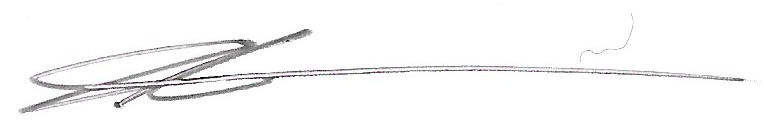
\includegraphics[height=0.78cm]{sonkiSignature}
  
\end{document}
